%! suppress = SentenceEndWithCapital
%! suppress = LineBreak
%! suppress = Unicode
%! suppress = MissingLabel
%! suppress = MissingImport
%! suppress = FileNotFound
\documentclass[../main.tex]{subfiles}

\begin{document}

    \subsection{Pokrycia logiczne}

    \begin{figure}[H]
        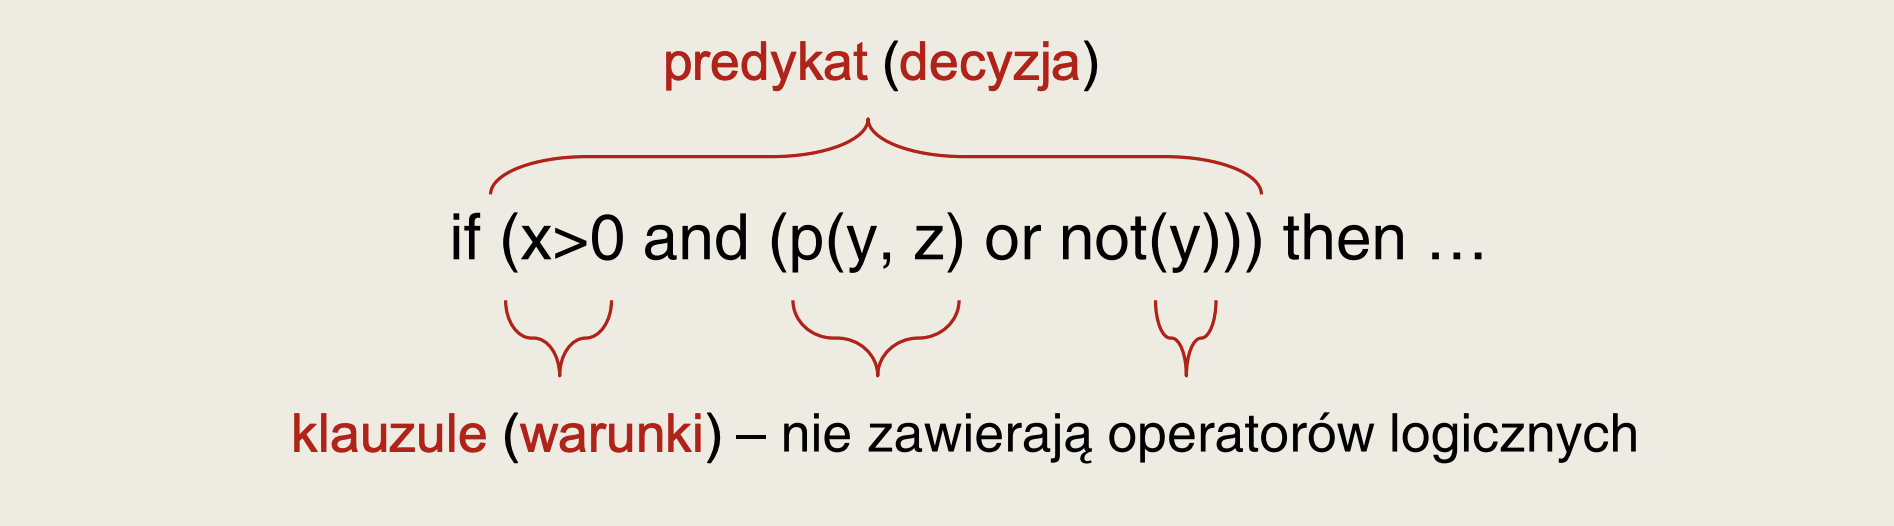
\includegraphics[width=\linewidth]{logika.png}
    \end{figure}

    \textbf{Problemy związane z pokryciem logicznym}
    \begin{itemize}
        \item \textbf{Problem sterowania} - jakie wartości x, y, z zadać, aby program wykonał się dokładnie taką ścieżką,
        jaką chcemy? Istnieją metody pomagające w tym, np. wykonanie symboliczne kodu (np. KLEE).


        \item \textbf{Problem zwarcia} - zwarcie to optymalizacja kompilatora pozwalająca szybciej ewaluować
        formuły logiczne (leniwa ewaluacja).
    \end{itemize}

    \subsubsection{Podstawowe kryteria}

    \begin{itemize}
        \item \textbf{Testowanie decyzji}
        \begin{itemize}
            \item rozważa decyzję jako niepodzielną całość
            \item każda \textbf{decyzja} musi \textbf{przynajmniej raz} przyjąć wartość TRUE i przynajmniej raz FALSE.
            \item praktycznie tożsame z \textbf{pokryciem krawędzi}.
        \end{itemize}

        \item \textbf{Testowanie warunków}
        \begin{itemize}
            \item rozważa \textbf{sposób ewaluacji decyzji}
            \item \textbf{każdy warunek} musi \textbf{przynajmniej raz} przyjąć wartość TRUE i przynajmniej raz wartość FALSE
        \end{itemize}

        \item \textbf{Testowanie wielokrotnych warunków}
        \begin{itemize}
            \item wymaga przetestowania \textbf{wszystkich możliwych kombinacji} wartości
            logicznych \textbf{warunków} tworzących decyzję
            \item wada: liczba testów jest wykładnicza względem liczby różnych
            warunków: dla N warunków musi być $2^N$ testów
            \item jeśli zachodzi \textbf{zwarcie}, liczba rzeczywistych testów może być zazwyczaj zredukowana.

        \end{itemize}
    \end{itemize}

    \begin{figure}[H]
        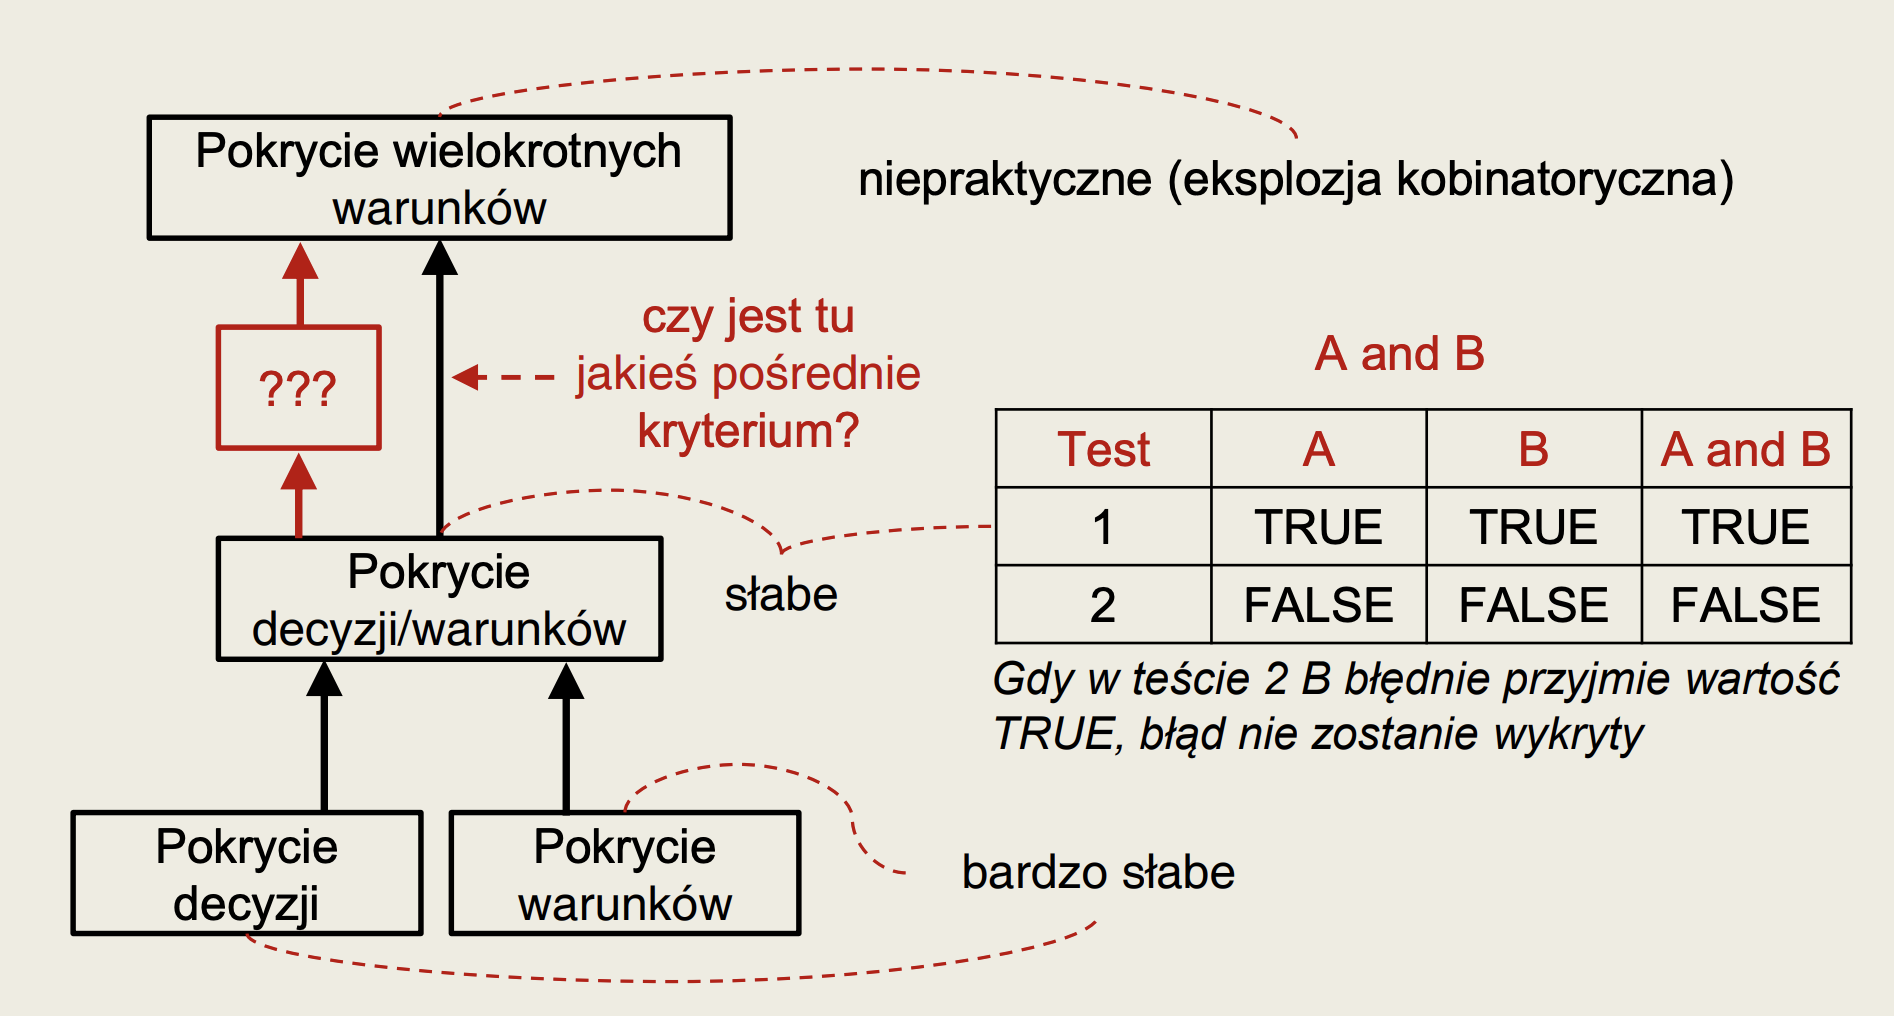
\includegraphics[width=\linewidth]{kryteria.png}
    \end{figure}

    \subsubsection{Kryterium MC/DC}

    \begin{itemize}
        \item słabsze niż wielokrotne warunki, ale silniejsze od warunków/decyzji
        \item dla \textbf{N} warunków wymaga zazwyczaj \textbf{N+1} testów (a więc liniowo)
        \item \textbf{wymaga dostarczenia takich testów, by każdy warunek pokazywał niezależnie swój wpływ na zmianę warunku
        logicznego decyzji}, tzn. dla każdego warunku W w decyzji D muszą istnieć 2 testy:
        \begin{itemize}
            \item W jest TRUE w jednym z nich i FALSE w drugim
            \item D jest TRUE w jednym z nich i FALSE w drugim
            \item wartości logiczne pozostałych warunków w tych dwóch testach
            nie zmieniają się
        \end{itemize}
        \item warunek W dla tych dwóch testów nazywany jest \textbf{klauzulą aktywną},
        a pozostałe warunki – \textbf{klauzulami pobocznymi}
        \item \textbf{Jak uczynić klauzulę aktywną?}
        \begin{itemize}
            \item niech D zawiera warunek A; chcemy, by A była klauzulą aktywną
            \item aby znaleźć wartości pozostałych warunków tak, by zmiana A wpływała
            na zmianę D, obliczamy D[A=TRUE] xor D[A=FALSE]
            \item wszystkie wartości logiczne dla pozostałych warunków, które spełniają
            powyższą formułę są dobrymi kandydatami
        \end{itemize}
    \end{itemize}

    \begin{figure}[H]
        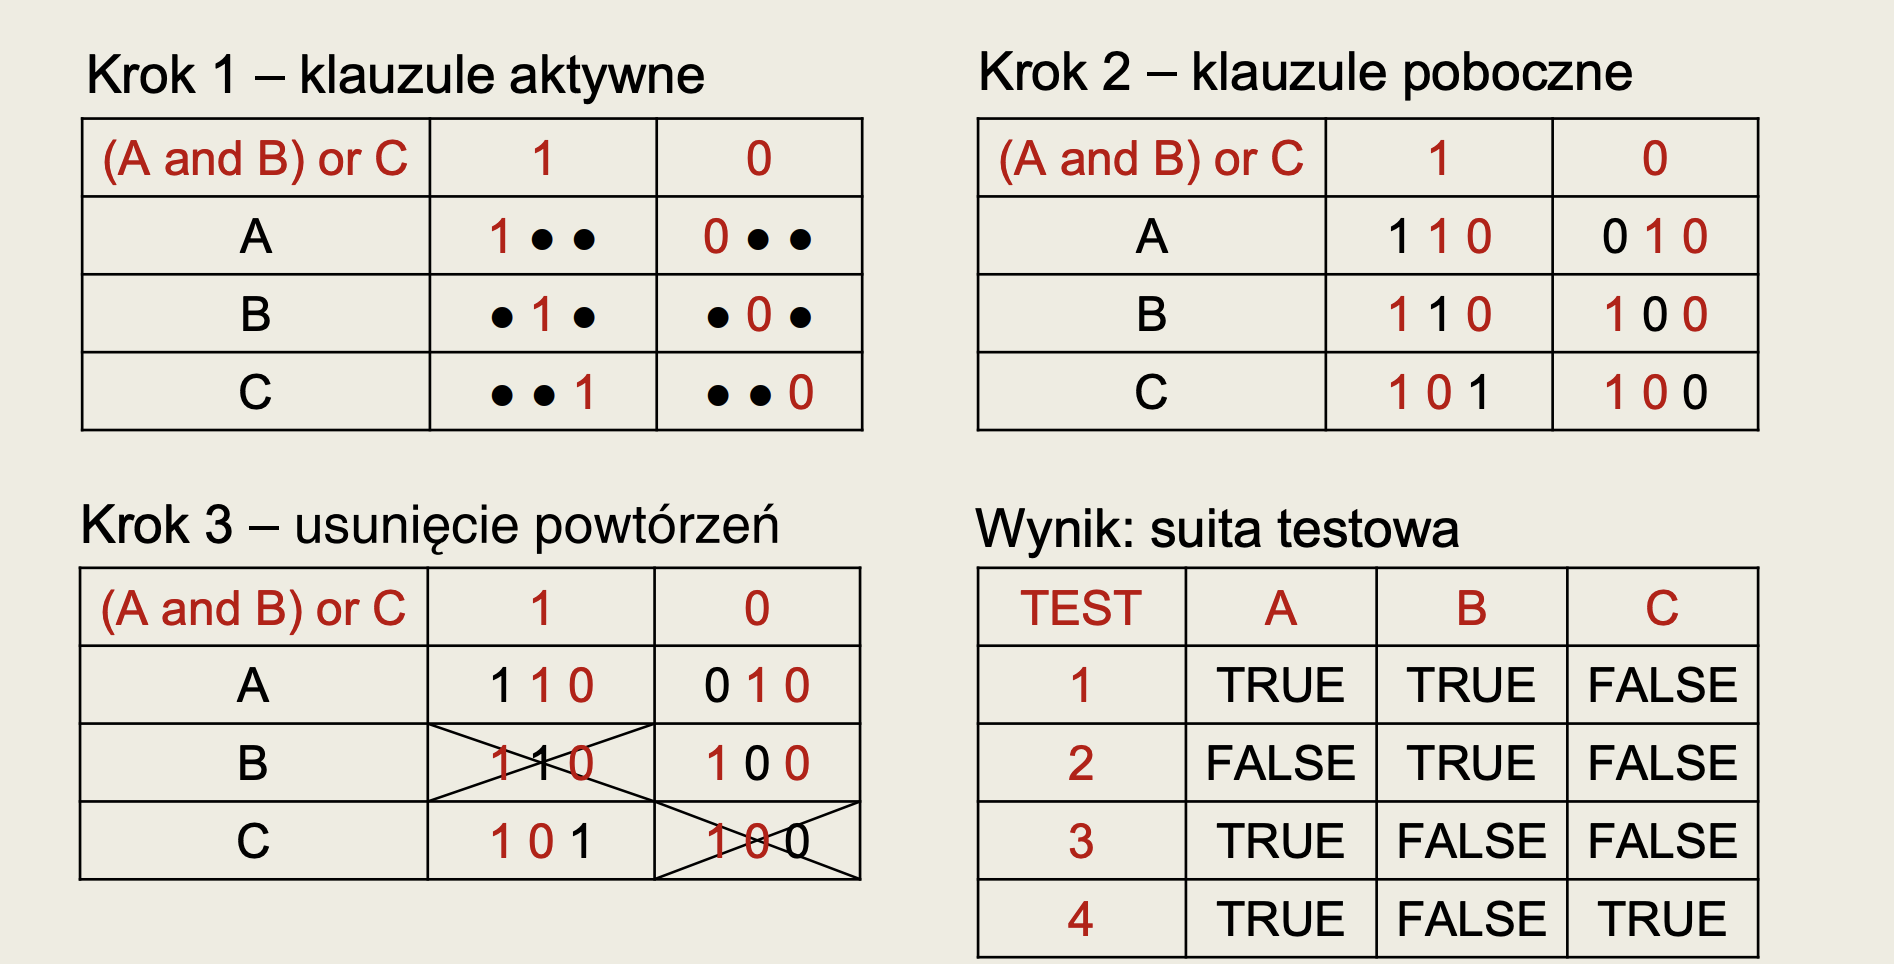
\includegraphics[width=\linewidth]{mcdc.png}
    \end{figure}

    \begin{table}[H]
        \begin{center}
            \begin{tabular}{p{8cm} p{8cm}}
                \textbf{Zalety}
                \begin{itemize}
                    \item \textbf{dobre kryterium pośrednie}
                    \item popularne w środowisku producentów awioniki (standard DO-178C)
                    \item \textbf{subsumuje pokrycie warunków/decyzji}, jednocześnie
                    wymagając tylko \textbf{liniowej} względem liczby klauzul liczby testów
                    \item dobra w znajdowaniu defektów takich jak:
                    \begin{itemize}
                        \item brakujący warunek, który powinien być obecny
                        \item AND błędnie zaimplementowany jako OR i vice versa
                        \item błędnie zaimplementowany operator relacyjny, np. < zamiast >
                    \end{itemize}
                    \item idea metody: \textbf{wykryje błąd}, gdy nastąpi \textbf{błędne wartościowanie jednego} (dowolnego!) z \textbf{warunków }decyzji
                \end{itemize}
                &
                \textbf{Wady}
                \begin{itemize}
                    \item \textbf{problematyczne}, jeśli występują tzw. \textbf{termy powiązane}
                    \begin{itemize}
                        \item może się nie dać spełnić warunku MC/DC
                        \item np. dla D = (A or B) and (not A) termy A i (not A) są powiązane
                        \item żadna wartość B nie pozwala A być klauzulą aktywną
                    \end{itemize}
                    \item możliwe rozwiązania:
                    \begin{itemize}
                        \item wymagać kryterium MC/DC jedynie dla termów niepowiązanych
                        \item analizować każdą decyzję zawierającą termy powiązane przypadek po przypadku
                    \end{itemize}
                    \item \textbf{problem zwarcia} (short-circuiting) może uniemożliwić osiągnięcie
                    odpowiedniego pokrycia MC/DC
                    \item \textbf{bardziej skomplikowane} niż słabsze kryteria
                    \begin{itemize}
                        \item na szczęście można \textbf{znajdować testy automatycznie}!
                    \end{itemize}
                \end{itemize}
            \end{tabular}
        \end{center}
    \end{table}
\end{document}